\documentclass[class=report,crop=false, 12pt]{standalone}
\usepackage[screen]{../myscratch}

\begin{document}


\titre[E]{Plusieurs lutins}
%===============================

\begin{enigme}[Paf le chien !]

Un chien et un chat courent l'un vers l'autre, où vont-ils se rencontrer ?


Sur le dessin, le chat se déplace de la gauche vers la droite, le chien de la droite vers la gauche.
\bigskip

\myfigure{0.8}{
\tikzinput{chien-chat-new}
}  



\textbf{Le chien.}
\begin{itemize}
  \item Il est réduit à une taille minuscule : le mettre à $0 \%$ de sa taille initiale.
  \item Il part de la position $(200,0)$, il s'oriente vers la gauche.
  \item Répéter indéfiniment : avancer de $3$.
\end{itemize}

\textbf{Le chat.}
\begin{itemize}
  \item Le mettre à $0 \%$ de sa taille initiale.
  \item Il part de la position $(-200,0)$, il s'oriente vers la droite.
  \item Répéter indéfiniment : avancer de $4$.
\end{itemize}


\bigskip

\textbf{Question.} Combien vaut l'abscisse $x$ de la position du chat lorsqu'il rencontre le chien ?
Arrondis la réponse à l'entier inférieur (une tolérance est acceptée !).


%\begin{solution}
%$x= 28$, donc réponse est 24,25,26,27,28,29,30,31,32.
%\end{solution}

\end{enigme}


%\begin{enigme}[Le chat course le chien !]
%
%Un chien est poursuivi par un chat. Où le chat va-t-il le rattraper ?
%\begin{center}
%  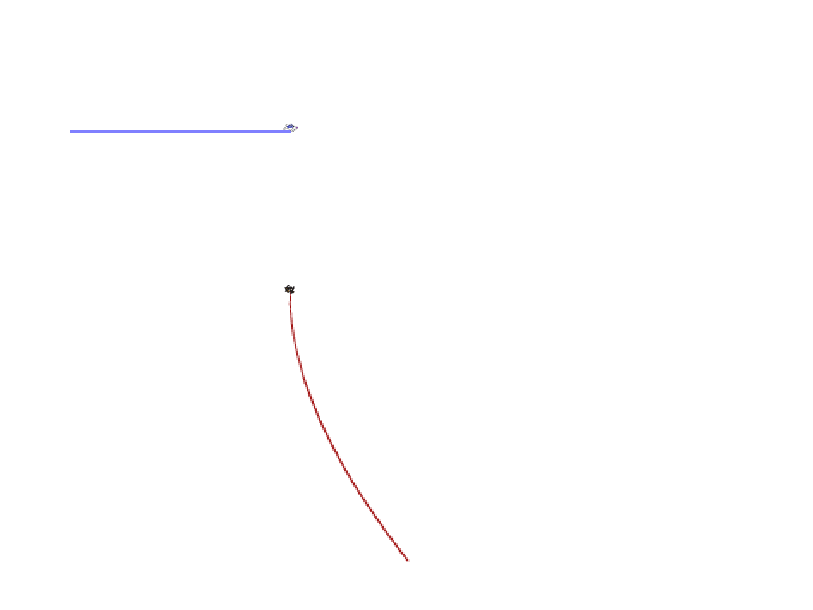
\includegraphics[scale=\scaleecran]{ecran-08-eg1} 
%\end{center}
%
%
%Sur le dessin, le chien se déplace horizontalement et a une trace bleue, le chat part du bas et a une trace rouge.
%
%Voici la position de départ :
%\myfigure{0.6}{
%\tikzinput{chien-chat}
%}  
%
%
%
%\textbf{Le chien.}
%\begin{itemize}
%  \item Il part de $(-200,100)$.
%  \item Il est réduit à une taille minuscule : le mettre à $0 \%$ de sa taille initiale.
%  \item Répéter indéfiniment : avancer de $3$.
%\end{itemize}
%
%\textbf{Le chat.}
%\begin{itemize}
%  \item Il part de $(0,-150)$.
%  \item Le mettre à $0 \%$ de sa taille initiale.
%  \item Répéter indéfiniment : 
%  \begin{itemize}
%    \item s'orienter vers le chien,
%    \item avancer de $4$.
%  \end{itemize}  
%\end{itemize}
%
%
%\bigskip
%
%\textbf{Question.} Combien vaut l'abscisse $x$ lorsque le chat rattrape le chien ?
%(Arrondir à l'entier inférieur ou supérieur.)
%
%
%%\begin{solution}
%%$x= 68.15$, donc réponse est $68$ ou $69$.
%%\end{solution}
%
%\end{enigme}





\begin{enigme}[Les chats de Fibonacci]

Un chat crée des clones de lui-même, qui eux-mêmes créent des clones\ldots
\begin{center}
  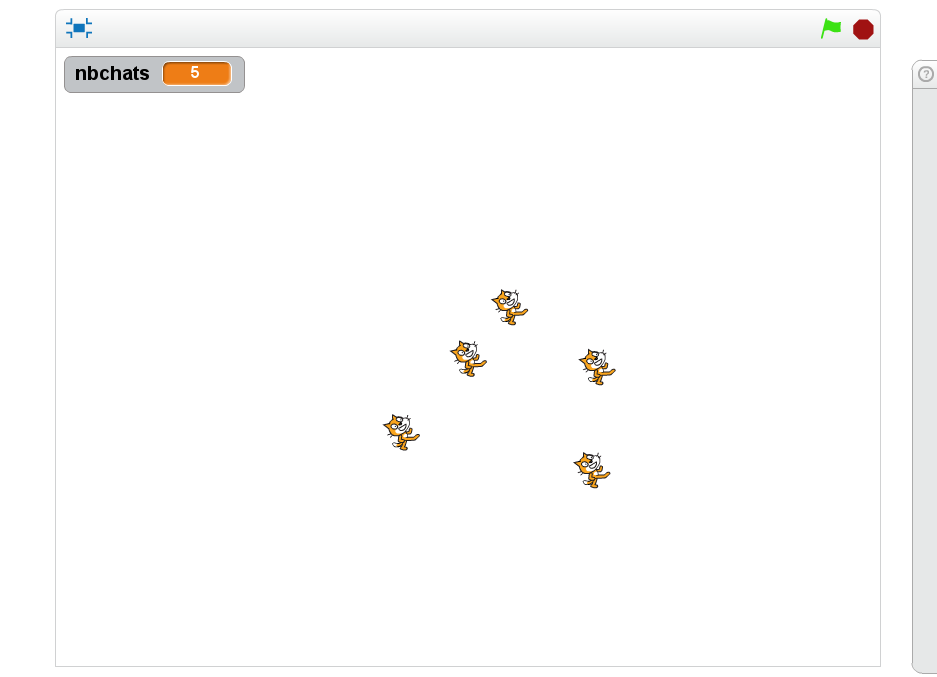
\includegraphics[width=0.6\textwidth]{ecran-08-eg2} 
\end{center}

\textbf{Le chat initial.}

Répéter $10$ fois :
\begin{itemize}
  \item Attendre $1$ seconde.
  \item Créer un clone de lui-même
\end{itemize}
Puis stopper tout.


\bigskip

\textbf{Les chats clonés.}

Quand un chat démarre comme un clone :
\begin{itemize}
  \item Attendre $1$ seconde, il se repose un peu !
  \item Répéter indéfiniment :
  \begin{itemize}
    \item Attendre $1$ seconde.
    \item Créer un clone de lui-même.
  \end{itemize}
\end{itemize}
  
\bigskip

On commence avec un chat, au bout d'une seconde
on a un chat et un clone. Au bout de $2$ secondes, le chat initial crée un nouveau clone, alors que le premier clone se repose encore un peu (on a donc $3$ chats en tout).
Au bout de $3$ secondes, on aura $2$ nouveaux chats (donc $5$ en tout)\ldots

\bigskip

\textbf{Question.} Combien de chats y a-t-il en tout au bout des $10$ secondes ?
\bigskip

\textbf{Blocs utiles.} 
\begin{itemize}
  \item Voici le bloc qui permet de créer un clone :
\begin{center}
\begin{scratch}
\blockcontrol{créer un clone de \ovalcontrol*{moi même}}
\end{scratch}
\end{center}

  \item Les instructions pour les clones débutent par le bloc suivant :
\begin{center}
\begin{scratch}
\blockinitclone{quand je commence comme un clone}
\end{scratch}
\end{center}
\end{itemize}

%\begin{solution}
%Suite de Fibonacci :
%$1,2,3,5,8,13,21,34,55,89,144$.
%Réponse : $144$.
%\end{solution}

\end{enigme}


\begin{enigme}[Le saut du chat]

Le chat effectue un saut et retombe dans la piscine (seul le début de sa trajectoire a été dessiné).

\begin{center}
  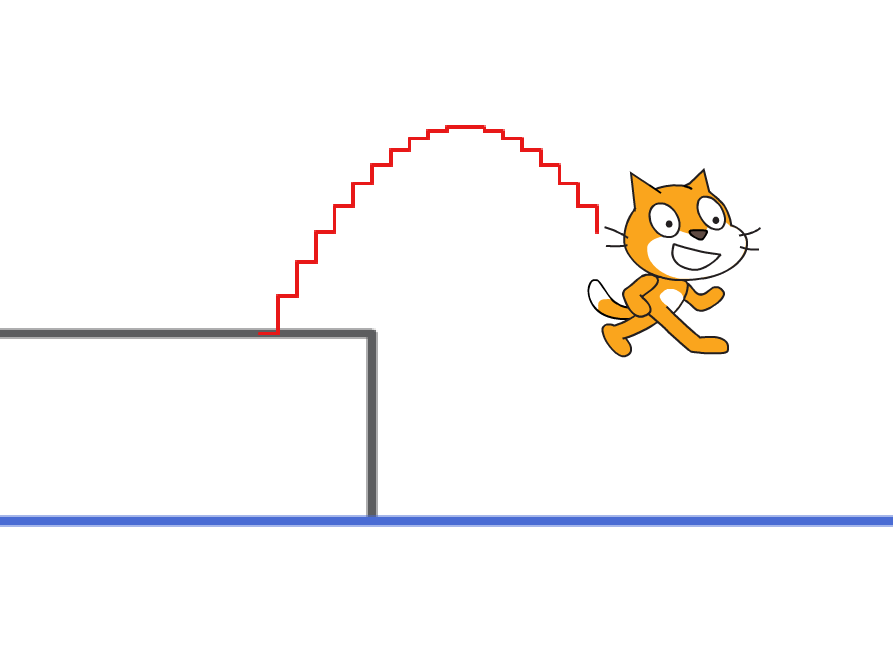
\includegraphics[width=0.6\textwidth]{ecran-08-eg3} 
\end{center}


\bigskip
\textbf{Le chat.}

\begin{itemize}
  \item Le chat part de la position $(-100,0)$.
  \item Le niveau de l'eau est $y=-100$.
  \item Il effectue un saut réaliste, comme décrit ci-dessous.
\end{itemize}


\bigskip
\textbf{Le saut réaliste.}

\begin{itemize}
  \item Une variable \codeinline{saut} est initialisée à $20$.
  \item On répète :
  \begin{itemize}
    \item ajouter $10$ à l'abscisse $x$,
    \item ajouter \codeinline{saut} à l'ordonnée $y$,
    \item ajouter $-2$ à \codeinline{saut}.
  \end{itemize}
\end{itemize}

\bigskip

\textbf{Question.} Combien de répétitions doivent être effectuées afin que le centre de Scratch touche l'eau ?


%\begin{solution}
%Réponse : nombre de répétitions est $25$. 
%\end{solution}

\end{enigme}

\end{document}

